\documentclass[11pt,letterpaper]{article}
\usepackage{graphicx}
\usepackage{multirow}
\usepackage{enumitem}
\usepackage{amssymb}
\usepackage{amsmath}
\usepackage{amsthm}
\usepackage{xcolor}
\usepackage{array}
\usepackage{geometry}
\usepackage{physics}
\usepackage{tikz}
\usepackage{tikz-3dplot}
\usetikzlibrary{arrows.meta, 3d}

\geometry{
    left = 15mm,
    right = 15mm,
    top = 20mm,
    bottom = 25mm,
}

\newcommand{\ihat}{\mathbf{i}}
\newcommand{\jhat}{\mathbf{j}}
\newcommand{\khat}{\mathbf{k}}

\begin{document}
\pagenumbering{gobble}

\begin{center}
  \textbf{\Large KUIS 2 ANALISIS VEKTOR (A)}\\
  Waktu : 100 menit\\
  Sifat : Tertutup
\end{center}

\vspace{0.5cm}

\begin{enumerate}
  \item Tentukan $\nabla \cdot \mathbf{F}$ dan $\nabla \times \mathbf{F}$ untuk
        \[
          \mathbf{F}(x,y,z)=e^{xy}\,\ihat-\cos y\,\jhat+\sin^2 z\,\khat.
        \]

        \textbf{Petunjuk:}\\
        Gunakan definisi divergensi dan curl.

  \item Tentukan apakah medan vektor berikut merupakan medan vektor konservatif. Jika ya, tentukan fungsi potensialnya.
        \[
          \mathbf{F}(x,y)=3y^2\,\ihat+6xy\,\jhat.
        \]

        \textbf{Petunjuk:}\\
        Untuk $\mathbf{F}(x,y)=P(x,y)\ihat+Q(x,y)\jhat$, periksa terlebih dahulu apakah
        \[
          \frac{\partial P}{\partial y}=\frac{\partial Q}{\partial x}.
        \]
        Jika syarat tersebut terpenuhi pada daerah yang diberikan, maka $\mathbf{F}$ merupakan medan vektor konservatif dan terdapat fungsi potensial $\phi(x,y)$ sehingga $\nabla \phi=\mathbf{F}$. Untuk menentukan fungsi potensial, gunakan
        \[
          \frac{\partial \phi}{\partial x}=P,
          \qquad
          \frac{\partial \phi}{\partial y}=Q.
        \]

  \item Gunakan Teorema Green untuk menghitung
        \[
          \oint_C 3xy\,dx+2xy\,dy,
        \]
        dengan $C$ adalah persegi panjang yang dibatasi oleh
        \[
          x=-2,\qquad x=4,\qquad y=1,\qquad y=2.
        \]

        \textbf{Petunjuk:}\\
        Gunakan Teorema Green
        \[
          \oint_C P\,dx+Q\,dy
          =
          \iint_D
          \left(
          \frac{\partial Q}{\partial x}
          -
          \frac{\partial P}{\partial y}
          \right)dA.
        \]

  \item Verifikasikan Teorema Stokes
        \[
          \oint_C \mathbf{F}\cdot d\mathbf{r}
          =
          \iint_\sigma (\nabla \times \mathbf{F})\cdot \mathbf{n}\,dS
        \]
        dengan menghitung integral garis dan integral permukaan secara langsung. Asumsikan bahwa permukaan memiliki orientasi ke atas (\textit{upward orientation}).
        \[
          \mathbf{F}(x,y,z)=x^2\ihat+y^2\jhat+z^2\khat,
        \]
        dengan $\sigma$ merupakan bagian kerucut
        \[
          z=\sqrt{x^2+y^2}
        \]
        yang berada di bawah bidang $z=1$.

        \textbf{Petunjuk:}
        \begin{enumerate}[label=(\alph*)]
          \item Tentukan kurva batas $C$ dan parameterisasinya.
          \item Hitung integral garis
                \[
                  \oint_C \mathbf{F}\cdot d\mathbf{r}.
                \]
          \item Hitung $\nabla \times \mathbf{F}$ dan tentukan vektor normal permukaan yang berorientasi ke atas.
          \item Hitung integral permukaan
                \[
                  \iint_\sigma (\nabla \times \mathbf{F})\cdot \mathbf{n}\,dS.
                \]
          \item Verifikasikan bahwa kedua hasil tersebut sama.
        \end{enumerate}

  \item Gunakan Teorema Divergensi (Gauss) untuk menentukan fluks keluar medan vektor
        \[
          \mathbf{F}(x,y,z)=x^3\ihat+y^3\jhat+z^3\khat
        \]
        melalui permukaan yang membatasi daerah hemisfer
        \[
          z=\sqrt{a^2-x^2-y^2}
        \]
        dan bidang $z=0$.

        \begin{center}
          \tdplotsetmaincoords{70}{110}
          \begin{tikzpicture}[tdplot_main_coords, scale=1.65]
            \draw[-Latex] (-1.5,0,0) -- (1.5,0,0) node[left] {$x$};
            \draw[-Latex] (0,-1.5,0) -- (0,1.5,0) node[right] {$y$};
            \draw[-Latex] (0,0,-0.5) -- (0,0,1.5) node[above] {$z$};

            \draw[thick, blue, fill=gray, opacity=0.2]
            plot[domain=0:360,smooth,variable=\t] ({cos(\t)},{sin(\t)},0);

            \foreach \ang in {0,1,...,180}{
                \draw[cyan, opacity=0.3] plot[domain=-90:90,smooth,variable=\t] ({cos(\ang)*sin(\t)},{sin(\ang)*sin(\t)},{cos(\t)});
              }

            \foreach \z/\r in {0.25/0.968,0.5/0.866,0.75/0.661}{
                \draw[cyan, opacity=0.25] plot[domain=0:360,smooth,variable=\t] ({\r*cos(\t)},{\r*sin(\t)},\z);
              }

            \draw[thick, blue] plot[domain=0:45,smooth,variable=\t] ({cos(\t)},{sin(\t)},0);
            \draw[thick, blue] plot[domain=45:360,smooth,variable=\t] ({cos(\t)},{sin(\t)},0);
          \end{tikzpicture}

          \vspace{0.2cm}
          \textbf{Gambar 1. Daerah hemisfer.}
        \end{center}

        \textbf{Petunjuk:}\\
        Gunakan Teorema Divergensi (Gauss)
        \[
          \iint_S \mathbf{F}\cdot \mathbf{n}\,dS
          =
          \iiint_V (\nabla \cdot \mathbf{F})\,dV.
        \]
        Hitung divergensinya terlebih dahulu. Untuk daerah hemisfer (Gambar 1), koordinat bola dapat digunakan:
        \[
          x=\rho\sin\phi\cos\theta,\qquad
          y=\rho\sin\phi\sin\theta,\qquad
          z=\rho\cos\phi,
        \]
        dengan
        \[
          dV=\rho^2\sin\phi\,d\rho\,d\phi\,d\theta.
        \]
\end{enumerate}

\newpage
\begin{center}
  \textbf{\Large SOLUSI}
\end{center}

\begin{enumerate}
  \item Diketahui
        \[
          \mathbf{F}(x,y,z)=e^{xy}\,\ihat-\cos y\,\jhat+\sin^2 z\,\khat.
        \]
        Misalkan
        \[
          P=e^{xy},\qquad Q=-\cos y,\qquad R=\sin^2 z.
        \]
        Divergensinya adalah
        \begin{flalign*}
          \nabla \cdot \mathbf{F}
           & =
          \frac{\partial P}{\partial x}
          +
          \frac{\partial Q}{\partial y}
          +
          \frac{\partial R}{\partial z}      \\
           & = ye^{xy}+\sin y+2\sin z\cos z.
        \end{flalign*}
        Jadi
        \[
          \boxed{\nabla \cdot \mathbf{F}=ye^{xy}+\sin y+2\sin z\cos z}.
        \]

        Curl-nya adalah
        \begin{flalign*}
          \nabla \times \mathbf{F}
           & =
          \begin{vmatrix}
            \ihat                       & \jhat                       & \khat                       \\
            \frac{\partial}{\partial x} & \frac{\partial}{\partial y} & \frac{\partial}{\partial z} \\
            e^{xy}                      & -\cos y                     & \sin^2 z
          \end{vmatrix} \\
           & =
          \left(
          \frac{\partial R}{\partial y}
          -
          \frac{\partial Q}{\partial z}
          \right)\ihat
          -
          \left(
          \frac{\partial R}{\partial x}
          -
          \frac{\partial P}{\partial z}
          \right)\jhat
          +
          \left(
          \frac{\partial Q}{\partial x}
          -
          \frac{\partial P}{\partial y}
          \right)\khat                                                                              \\
           & = (0-0)\ihat-(0-0)\jhat+(0-xe^{xy})\khat.
        \end{flalign*}
        Maka
        \[
          \boxed{\nabla \times \mathbf{F}=-xe^{xy}\,\khat}.
        \]

  \item Diketahui
        \[
          \mathbf{F}(x,y)=3y^2\,\ihat+6xy\,\jhat.
        \]
        Misalkan $P=3y^2$ dan $Q=6xy$. Periksa syarat konservatif:
        \[
          \frac{\partial P}{\partial y}=6y,
          \qquad
          \frac{\partial Q}{\partial x}=6y.
        \]
        Karena
        \[
          \frac{\partial P}{\partial y}
          =
          \frac{\partial Q}{\partial x},
        \]
        maka $\mathbf{F}$ adalah medan vektor konservatif pada $\mathbb{R}^2$.

        Selanjutnya cari fungsi potensial $\phi(x,y)$ sehingga $\nabla \phi=\mathbf{F}$. Dari
        \[
          \frac{\partial \phi}{\partial x}=3y^2,
        \]
        diperoleh
        \[
          \phi(x,y)=3xy^2+g(y).
        \]
        Turunkan terhadap $y$:
        \[
          \frac{\partial \phi}{\partial y}=6xy+g'(y).
        \]
        Karena harus sama dengan $Q=6xy$, maka
        \[
          6xy+g'(y)=6xy
          \implies
          g'(y)=0.
        \]
        Jadi $g(y)=C$. Dengan demikian fungsi potensialnya adalah
        \[
          \boxed{\phi(x,y)=3xy^2+C}.
        \]

  \item
        Diketahui
        \[
          P=3xy,
          \qquad
          Q=2xy.
        \]
        Dengan Teorema Green,
        \[
          \oint_C P\,dx+Q\,dy
          =
          \iint_D
          \left(
          \frac{\partial Q}{\partial x}
          -
          \frac{\partial P}{\partial y}
          \right)dA.
        \]
        Hitung turunan parsialnya:
        \[
          \frac{\partial Q}{\partial x}=2y,
          \qquad
          \frac{\partial P}{\partial y}=3x.
        \]
        \begin{center}
          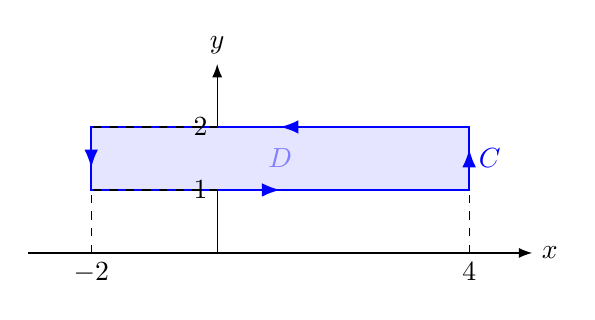
\begin{tikzpicture}[scale=0.8]
            \draw[-Latex] (-3,0) -- (5,0) node[right] {$x$};
            \draw[-Latex] (0,0) -- (0,3) node[above] {$y$};
            \draw[fill=blue!10, draw=blue, thick] (-2,1) rectangle (4,2);
            \draw[blue, thick, -Latex] (-2,1) -- (1,1);
            \draw[blue, thick, -Latex] (4,1) -- (4,1.65);
            \draw[blue, thick, -Latex] (4,2) -- (1,2);
            \draw[blue, thick, -Latex] (-2,2) -- (-2,1.35);
            \node[below] at (-2,0) {$-2$};
            \node[below] at (4,0) {$4$};
            \node[left] at (0,1) {$1$};
            \node[left] at (0,2) {$2$};
            \node[blue!50] at (1,1.5) {$D$};
            \node[blue, right] at (4,1.5) {$C$};
            \draw[dashed] (-2,0) -- (-2,1);
            \draw[dashed] (4,0) -- (4,1);
            \draw[dashed] (0,1) -- (-2,1);
            \draw[dashed] (0,2) -- (-2,2);
          \end{tikzpicture}
        \end{center}
        Karena daerah $D$ adalah persegi panjang
        \[
          -2\le x\le 4,
          \qquad
          1\le y\le 2,
        \]
        maka
        \begin{flalign*}
          \oint_C 3xy\,dx+2xy\,dy
           & =
          \int_{-2}^{4}\int_{1}^{2}(2y-3x)\,dy\,dx \\
           & =
          \int_{-2}^{4}
          \left[
            y^2-3xy
            \right]_{1}^{2}
          dx                                       \\
           & =
          \int_{-2}^{4}
          \left(
          4-6x-1+3x
          \right)dx                                \\
           & =
          \int_{-2}^{4}(3-3x)\,dx                  \\
           & =
          \left[
            3x-\frac{3}{2}x^2
            \right]_{-2}^{4}                       \\
           & =
          (12-24)-\left(-6-6\right)=0.
        \end{flalign*}
        Jadi
        \[
          \boxed{\oint_C 3xy\,dx+2xy\,dy=0}.
        \]

  \item Permukaan $\sigma$ adalah bagian kerucut
        \[
          z=\sqrt{x^2+y^2}
        \]
        di bawah bidang $z=1$. Irisannya dengan bidang $z=1$ memenuhi
        \[
          1=\sqrt{x^2+y^2}
          \implies
          x^2+y^2=1.
        \]
        \begin{center}
          \tdplotsetmaincoords{70}{120}
          \begin{tikzpicture}[tdplot_main_coords, scale=2]
            \draw[-Latex] (-1.3,0,0) -- (1.4,0,0) node[below] {$x$};
            \draw[-Latex] (0,-1.3,0) -- (0,1.4,0) node[right] {$y$};
            \draw[-Latex] (0,0,0) -- (0,0,1.5) node[above] {$z$};

            \foreach \ang in {0,1,...,330}{
                \draw[cyan!60] (0,0,0) -- ({cos(\ang)},{sin(\ang)},1);
              }
            \draw[fill=cyan!20, fill opacity=0.45, draw=cyan!70!black, thick]
            plot[domain=0:360, smooth, variable=\t] ({cos(\t)},{sin(\t)},1) -- (0,0,0) -- cycle;
            \draw[cyan!70!black, thick]
            plot[domain=0:360, smooth, variable=\t] ({cos(\t)},{sin(\t)},1);
            \draw[blue, thick, -Latex]
            plot[domain=25:385, smooth, variable=\t] ({cos(\t)},{sin(\t)},1);
            \node[blue, right] at (0,1,1) {$C$};

            \draw (0,0,0.65) -- (0,0,1.4);
          \end{tikzpicture}
        \end{center}
        Jadi kurva batasnya adalah lingkaran
        \[
          C:\quad x^2+y^2=1,\quad z=1.
        \]
        Karena orientasi permukaan ke atas, orientasi positif $C$ adalah berlawanan arah jarum jam jika dilihat dari atas. Parameterisasi kurva batas:
        \[
          \mathbf{r}(t)=(\cos t,\sin t,1),
          \qquad
          0\le t\le 2\pi.
        \]
        Maka
        \[
          \mathbf{r}'(t)=(-\sin t,\cos t,0).
        \]
        Pada $C$,
        \[
          \mathbf{F}(\mathbf{r}(t))
          =
          \cos^2 t\,\ihat+\sin^2 t\,\jhat+\khat.
        \]
        Integral garisnya:
        \begin{flalign*}
          \oint_C \mathbf{F}\cdot d\mathbf{r}
           & =
          \int_{0}^{2\pi}
          \mathbf{F}(\mathbf{r}(t))\cdot \mathbf{r}'(t)\,dt \\
           & =
          \int_{0}^{2\pi}
          \left(
          \cos^2 t,\sin^2 t,1
          \right)
          \cdot
          \left(
          -\sin t,\cos t,0
          \right)dt                                         \\
           & =
          \int_{0}^{2\pi}
          \left(
          -\cos^2 t\sin t+\sin^2 t\cos t
          \right)dt                                         \\
           & =
          \left[
            \frac{1}{3}\cos^3 t+\frac{1}{3}\sin^3 t
            \right]_{0}^{2\pi}=0.
        \end{flalign*}

        Selanjutnya,
        \[
          \nabla \times \mathbf{F}
          =
          \begin{vmatrix}
            \ihat                       & \jhat                       & \khat                       \\
            \frac{\partial}{\partial x} & \frac{\partial}{\partial y} & \frac{\partial}{\partial z} \\
            x^2                         & y^2                         & z^2
          \end{vmatrix}
          =
          \mathbf{0}.
        \]
        Untuk menghitung langsung integral permukaan, parameterisasikan kerucut dengan
        \[
          \mathbf{r}(r,\theta)
          =
          (r\cos\theta,r\sin\theta,r),
          \qquad
          0\le r\le 1,\quad 0\le \theta\le 2\pi.
        \]
        Diperoleh
        \[
          \mathbf{r}_r=(\cos\theta,\sin\theta,1),
          \qquad
          \mathbf{r}_\theta=(-r\sin\theta,r\cos\theta,0).
        \]
        Vektor normal berorientasi ke atas dapat diambil
        \[
          \mathbf{r}_r\times \mathbf{r}_\theta
          =
          (-r\cos\theta,-r\sin\theta,r),
        \]
        karena komponen $z$-nya positif. Maka
        \begin{flalign*}
          \iint_\sigma
          (\nabla\times \mathbf{F})\cdot \mathbf{n}\,dS
           & =
          \int_{0}^{2\pi}\int_{0}^{1}
          \mathbf{0}\cdot
          (-r\cos\theta,-r\sin\theta,r)
          \,dr\,d\theta =0.
        \end{flalign*}
        Jadi
        \[
          \boxed{
            \oint_C \mathbf{F}\cdot d\mathbf{r}=0
            =
            \iint_\sigma
            (\nabla\times \mathbf{F})\cdot \mathbf{n}\,dS
          }.
        \]
        Maka Teorema Stokes terverifikasi.

  \item Diketahui
        \[
          \mathbf{F}(x,y,z)=x^3\ihat+y^3\jhat+z^3\khat.
        \]
        Dengan Teorema Divergensi,
        \[
          \iint_S \mathbf{F}\cdot \mathbf{n}\,dS
          =
          \iiint_V (\nabla \cdot \mathbf{F})\,dV.
        \]
        Hitung divergensinya:
        \[
          \nabla \cdot \mathbf{F}
          =
          \frac{\partial}{\partial x}(x^3)
          +
          \frac{\partial}{\partial y}(y^3)
          +
          \frac{\partial}{\partial z}(z^3)
          =
          3x^2+3y^2+3z^2.
        \]
        Dalam koordinat bola,
        \[
          x^2+y^2+z^2=\rho^2,
        \]
        sehingga
        \[
          \nabla \cdot \mathbf{F}=3\rho^2.
        \]
        Daerah hemisfer atas berjari-jari $a$ memiliki batas
        \[
          0\le \rho\le a,
          \qquad
          0\le \phi\le \frac{\pi}{2},
          \qquad
          0\le \theta\le 2\pi.
        \]
        Maka fluks keluar adalah
        \begin{flalign*}
          \iint_S \mathbf{F}\cdot \mathbf{n}\,dS
           & =
          \int_{0}^{2\pi}
          \int_{0}^{\pi/2}
          \int_{0}^{a}
          3\rho^2
          \rho^2\sin\phi
          \,d\rho\,d\phi\,d\theta               \\
           & =
          3
          \left[
            \frac{\rho^5}{5}
            \right]_{0}^{a}
          \left[
            -\cos\phi
            \right]_{0}^{\pi/2}
          \left[
            \theta
            \right]_{0}^{2\pi}                  \\
           & =
          3\cdot \frac{a^5}{5}\cdot 1\cdot 2\pi \\
           & =
          \boxed{\frac{6\pi a^5}{5}}.
        \end{flalign*}
\end{enumerate}

\end{document}
